\chapter{Introduction} % (fold)
\label{cha:introduction}
Twitter is a mircoblogging service which is used by millions users. Users can publish and exchange information with short tweets within 140 characters. It is cheap and can be accessed though several types clients like website, email or mobile phone. Those advantages make Titter agile and simple to use.  A study by the Pew Research Center shows that the people in USA under age of 30 consider Internet becomes the major resource of news and in all ages crowds Internet became the second important media \cite{kohut2008internet}.

But these advantages make Twitter become one of the most importance resources of breaking news, at the same time it becomes into a ideal media for spreading unverified information. On Twitter everyone can be a journalist and publish news or rumors without any substantiation which must be done by traditional journalists before news' publishing. 

 Rumor could be defined as a statement whose truth value is unverified or deliberately false \cite{qazvinian2011rumor}. And they could be harmful to the government, market and society. One case is some hacked accounts spread a rumor about Obama had been injured in white house. The S\&P crashed and wiped off 130 Billion dollars of stock value \cite{matthews2013does}. 
 
 So a method of detecting rumors on Twitter can be very useful and it will better it can detect rumors so soon as possible before it widely spreads.    
 The structure is shown in figure \ref{fig:pipeline}. First 1) we crawled the data from Twitter interface, 2) we use beautiful soup and spark technologies to extract feature from the tweets, 3) we extract time series features and fit to the dynamic series-time structure 4) we use the text of tweets as feature to train the single tweet's credibility scoring model neural network and merge the its output to the time series features, 5) training the our time series model with DSTS.  
 
 \begin{figure}[!h]
\centering
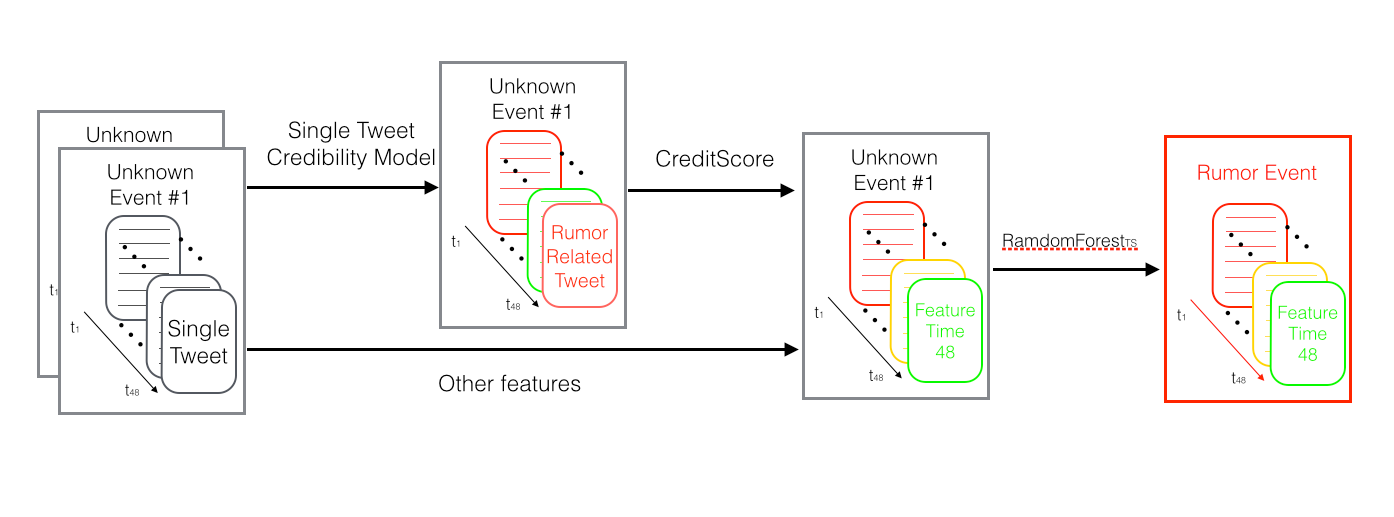
\includegraphics[width=\columnwidth]{images/structuremodel.png}
\caption{ pipeline of the rumor detecting system }
\label{fig:pipeline}
\end{figure}

 \newpage
 \subsection{Contributions}
In this thesis, we make the following contributions:

\begin{itemize}
	\item We are the first research which clearly defines the time period of rumor events. Other works either use natural time period like June of 2012 or didn't explain their definition. We develop the method of definition of rumor's time period in section \ref{sec:Time_Period_of_an_Event}. 
	\item We develop a model of classification of single tweet with high credibility or low credibility. We call it \textsc{single tweet's creditability scoring model}. Considering it could be set up online for the early rumor events detection in the further and it should response as quick as possible. So we use only the features which can be extracted from one tweet in the Twitter's interface. We test 2 models. One is random decision forest with handcrafted features. Because the features are limited, it gets only 64\% accuracy. Second model what we tested is based on zhou's\cite{zhou2015c} work, it is a hybrid CNN and LSTM model for text classification. The result of this model we called it credit score with 81\% accuracy.

 	\item We develop a time series model for detecting rumor events. We used Dynamic Series-Time Structure (DSTS)\cite{liu2015real} to capture the changes of features over time. And we tested 3 time series model as feature: modified Spike Model \cite{kwon2013prominent}, SIS model and SEIZ model\cite{jin2013epidemiological}. We add the results of credit scoring model as a feature into time series model to improve the performance in the early stage. And we approved that credit score is one of the best feature in the rumor detection task. In 48 hours after the event's spreading we got 90\% accuracy to detect the rumor events. 

 	\item We study how the performances of features change over time during the spreading of rumors. For example the performance of features of external URLs gets better after 24 hours and the features of sentiments are useless after 25 hours.  And within 25 hours which is average time for human editors detecting rumors we get 87\% accuracy.

 \end{itemize}
 
 
\subsection{Thesis Outline}

The rest of this these is organized as follows: In Chapter~\ref{cha:Related_Work} we explain some terminology of Twitter and some techniques which we use for extracting feature and modeling. in Chapter~\ref{cha:single_tweet_creditbility_scoring_model}, we introduce our single tweet credibility model. We show the performance of models with handcrafted features are worse than the neutral network model. In\ref{cha:timr_seriers_rumor_model}, we mainly introduce the time series model and its time series features. We compare the time series model and static model and we discuss the performance of features changing over time. Finally, in Chapter~\ref{cha:conclusion_and_future_work} we add some concluding remarks and describe future work.

% chapter introduction (end)